
%\documentclass[10pt,twoside,twocolumn]{article}
\documentclass[12pt,twoside]{article}
\usepackage[bf,small]{caption}
\usepackage[letterpaper,hmargin=1in,vmargin=1in]{geometry}
\usepackage{paralist} % comapctitem, compactdesc, compactenum
\usepackage{titlesec}
\usepackage{titletoc}
\usepackage{times}
\usepackage{hyperref}
\usepackage{algorithmic}
\usepackage{graphicx}
\graphicspath{{./graphics/}}
\usepackage{xspace}
\usepackage{verbatim}
\usepackage{url}
\usepackage{float}
\hyphenation{Sub-Bytes Shift-Rows Mix-Col-umns Add-Round-Key}

\setlength{\parskip}{12pt}
\setlength{\parindent}{0pt}

\newcommand{\hdb}{\emph{hashdb}\xspace}
\newcommand{\bulk}{\emph{bulk\_extractor}\xspace}
\newcommand{\hashid}{\emph{hashid}\xspace}
\newcommand{\mdd}{\emph{md5deep}\xspace}
\newcommand{\bev}{\emph{Bulk Extractor Viewer}\xspace}

\begin{document}

\begin{center}
\Large Demo: Preparing a Block Hash Database \\
\large Using \mdd and \hdb
\end{center}

We build large block hash databases to help us find specific data.
\begin{compactitem}
\item We search a database of blacklist hashes to find blocks
that are from blacklisted data.
\item We subtract hashes that match whitelist data
to remove obvious false positives.
\end{compactitem}
The Scanner demo at
\url{www.digitalcorpora.org/downloads/hashdb/scanner\_demo.pdf}.
references a database of blacklisted hash values
to find that a media image contains part of a blacklisted video file.

The Similarity demo at
\url{www.digitalcorpora.org/downloads/hashdb/similarity\_demo.pdf}.
subtracts whitelist hash values
to reveal user files that are common in two media images.

The workflow for managing blacklist databases and whitelist databases
is the same:
\begin{compactenum}
\item Generate block hash values in DFXML format
from blacklist or whitelist sources.
\item Import these block hash values into a \hdb hash database.
%\item Tailor the contents of a database by adding or removing
%specific hash values.
\end{compactenum}

%Here is the workflow:
Generate block hashes in DFXML format:

\begin{figure}[H]
  \center
  
\includegraphics[scale=0.6]{drawings/md5deep}
  \caption*{Run \mdd to create a DFXML file of block hashes \\
            from your library of blacklist or whitelist files.}
\end{figure}

Import block hashes into the hash database:

\begin{figure}[H]
  \center
  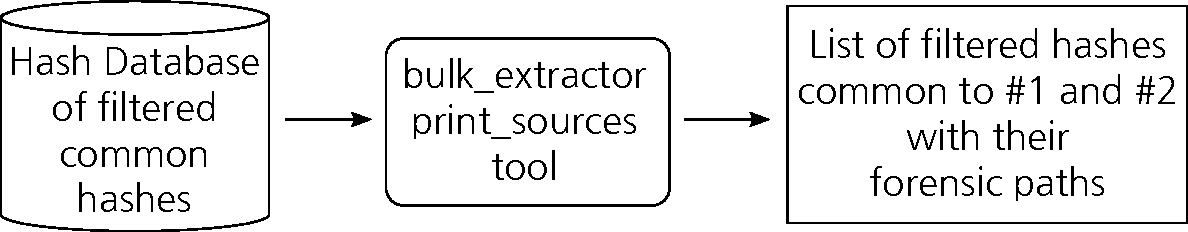
\includegraphics[scale=0.6]{drawings/import}
  \caption*{Run the \hdb \texttt{import} command
            to import block hashes into the hash database.}
\end{figure}

%Use \hdb tool commands to tailor your database as needed.
%For example:
%\begin{compactenum}
%\item If a hash 
%\end{compactenum}

%steps
Here are the steps to perform this demo:
\textbf{NOTE: These downloads and \hdb v1.0.0 are not available yet.}
\begin{compactenum}
\item Download and install \hdb from
\url{www.digitalcorpora.org/downloads/hashdb/hashdb-1.0.0\_beta-windowsinstaller.exe}.
\item Download and install \bulk compiled with \hdb from
\url{www.digitalcorpora.org/downloads/hashdb/bulk\_extractor-1.4.4-windowsinstaller.exe}
\item Pick a directory to use as your source of whitelist or blacklist files.
For example pick your \texttt{Downloads} directory.

\item Use the \mdd tool to generate the DFXML file of block hashes
of your \texttt{Downloads} directory.
\begin{compactitem}
\item Use \texttt{-p 4096} to specify a block (partition) size of 4096.
\item Use \texttt{-d} to generate output in DFXML format.
\item Use \texttt{-r} to generate block hashes recursively in subdirectories.
\item Use \texttt{> my\_dfxml\_file} to direct the DFXML output
to go to the \texttt{my\_dfxml\_file} file.
\end{compactitem}
\begin{verbatim}
$ md5deep -p 4096 -d -r Downloads > my_dfxml_file
\end{verbatim}

\item Use the \hdb tool to \texttt{create} the new hash database:
\begin{verbatim}
$ hashdb create my_blacklist_db
\end{verbatim}

\item Use the \hdb tool to \texttt{import} the block hashes
into the hash database:
\begin{verbatim}
$ hashdb import my_dfxml_file my_blacklist_db
\end{verbatim}
\end{compactenum}

\end{document}

